%header and footer for separate chapter files

\ifx\whole\undefined
\documentclass[12pt, leqno]{book}
\usepackage{graphicx}
\input style-for-curves.sty
\usepackage{hyperref}
\usepackage{showkeys} %This shows the labels.
%\usepackage{SLAG,msribib,local}
%\usepackage{amsmath,amscd,amsthm,amssymb,amsxtra,latexsym,epsfig,epic,graphics}
%\usepackage[matrix,arrow,curve]{xy}
%\usepackage{graphicx}
%\usepackage{diagrams}
%
%%\usepackage{amsrefs}
%%%%%%%%%%%%%%%%%%%%%%%%%%%%%%%%%%%%%%%%%%
%%\textwidth16cm
%%\textheight20cm
%%\topmargin-2cm
%\oddsidemargin.8cm
%\evensidemargin1cm
%
%%%%%%Definitions
%\input preamble.tex
%\input style-for-curves.sty
%\def\TU{{\bf U}}
%\def\AA{{\mathbb A}}
%\def\BB{{\mathbb B}}
%\def\CC{{\mathbb C}}
%\def\QQ{{\mathbb Q}}
%\def\RR{{\mathbb R}}
%\def\facet{{\bf facet}}
%\def\image{{\rm image}}
%\def\cE{{\cal E}}
%\def\cF{{\cal F}}
%\def\cG{{\cal G}}
%\def\cH{{\cal H}}
%\def\cHom{{{\cal H}om}}
%\def\h{{\rm h}}
% \def\bs{{Boij-S\"oderberg{} }}
%
%\makeatletter
%\def\Ddots{\mathinner{\mkern1mu\raise\p@
%\vbox{\kern7\p@\hbox{.}}\mkern2mu
%\raise4\p@\hbox{.}\mkern2mu\raise7\p@\hbox{.}\mkern1mu}}
%\makeatother

%%
%\pagestyle{myheadings}

%\input style-for-curves.tex
%\documentclass{cambridge7A}
%\usepackage{hatcher_revised} 
%\usepackage{3264}
   
\errorcontextlines=1000
%\usepackage{makeidx}
\let\see\relax
\usepackage{makeidx}
\makeindex
% \index{word} in the doc; \index{variety!algebraic} gives variety, algebraic
% PUT a % after each \index{***}

\overfullrule=5pt
\catcode`\@\active
\def@{\mskip1.5mu} %produce a small space in math with an @

\title{Personalities of Curves}
\author{\copyright David Eisenbud and Joe Harris}
%%\includeonly{%
%0-intro,01-ChowRingDogma,02-FirstExamples,03-Grassmannians,04-GeneralGrassmannians
%,05-VectorBundlesAndChernClasses,06-LinesOnHypersurfaces,07-SingularElementsOfLinearSeries,
%08-ParameterSpaces,
%bib
%}

\date{\today}
%%\date{}
%\title{Curves}
%%{\normalsize ***Preliminary Version***}} 
%\author{David Eisenbud and Joe Harris }
%
%\begin{document}

\begin{document}
\maketitle

\pagenumbering{roman}
\setcounter{page}{5}
%\begin{5}
%\end{5}
\pagenumbering{arabic}
\tableofcontents
\fi


\chapter{The Riemann-Roch Theorem}\label{RiemannRochChapter}

\subsection{Measuring linear series}

Because we are going to study curves via their maps to projective spaces, we will want to know how large a space of global
sections we should expect an invertible sheaf to have. We will answer this in several ways, but the beginning
of the story is the Riemann-Roch theorem.

We will henceforward assume that the reader is acquainted with sheaf cohomology, at least sufficiently to write
$H^i(X, \sF)$ without blushing. If $\sF$ is a sheaf on $X$ and $X\subset Y$ then we will identify $\sF$ with
the sheaf usually written $\iota_*\sF$, where $\iota:X\to Y$ is the inclusion map,
 and thus regard $\sF$ on as a sheaf on $Y$ as well.
The cohomology  $H^i(X, \sF) = H^i(Y,\iota_*\sF)$ canonically, so we will
simply and unambiguously write $H^i(\sF)$ for either of these. 
We write $h^i(\sF)$ or (if $D$ is a divisor) $h^{i}(D)$ for $\dim_{\CC}H^i(\sF)$ or $\dim_{\CC}H^i(D)$. 

Since we need lots of global sections of a line bundle $\sL$ to produce interesting maps from a curve $C$, we would like to be able to compute  $h^0(\sL) = \dim H^0(\sL)$. Much easier is to compute a sort of approximation to this number,
$$
\chi(\sL):= \sum_{i\geq 0} (-1)^i h^i(\sL),
$$
which makes sense, and even computes $h^0(\cL)$ itself in many cases, by virtue of the following result:

\begin{theorem} (Vanishing Theorem)\label{Serre-Grothendieck vanishing}
If $\sF$ is a coherent sheaf on a scheme $X$ of dimension $n$, then for any $i$, the vector space $H^i(\sF)$ is finite dimensional, and 0 if  $i>\dim X$. Moreover,
if $X\subset \PP^m$, then $H^i(\sF(d)) = 0$ for all $i>0$ and $d\gg 0$.\qed
\end{theorem}

\begin{proof}
This is a combination of Theorems \cite[Theorems III.2.7 and III.5.2]{Hartshorne1977}, due to Grothendieck and Serre.
\end{proof}

Thus on a scheme $X\subset \PP^r$ we have $\chi(\sL(d)) = h^0(\sL(d))$ for large $d$, and in the case of a curve $C\subset \PP^r$, we have $\chi(\sL) = h^0(\sL) - h^1(\sL)$.

\begin{theorem} (Easy Riemann-Roch)\label{easy RR}
If $C$ is a smooth curve, and $\sL$ is an invertible sheaf on $C$, then $\chi(\sL) = \deg \sL + \chi(\sO_C)$.
\end{theorem}

\begin{proof}
 The result is tautological if $\sL = \sO_C$. Every invertible sheaf on $C$ has the form $\sL = \sO_C(D)$ for some
divisor $D$. If $p\in C$, then writing $\kappa(p)$ for the 1-dimensional skyscraper sheaf at $p$, the long exact sequence in cohomology
associated to the short exact sequence
$$
0\to \sL(-p) \to \sL \to \sL\otimes \kappa(p)\to 0
$$
together with the isomorphism $\sL\otimes \kappa(p) \cong \kappa(p)$
and the vanishing of higher cohomology of a sheaf with zero-dimensional support allows us to compute 
$$
\chi(\sL) = \chi(\sL(-p)) + \chi(\kappa(p)) = \chi(\sL(-p)) + 1.
$$
Since every divisor on $C$ can be reached by adding and subtracting points, this suffices.
\end{proof}

We can make a more useful Riemann-Roch theorem by understanding the error term $h^1(\sL)$ using
the canonical divisor and Serre duality, to which
we now turn.


\section{The most interesting linear series}

The most important vector bundles on a manifold are the tangent and cotangent bundles. For reasons that
will become clear, the focus in algebraic geometry is on the cotangent bundle or, equivalently, the sheaf of differential forms. On a smooth curve $C$, this is usually called the \emph{canonical sheaf}; on a smooth
variety of dimension $n$ the canonical sheaf is the $n$-exterior power of the sheaf of differentials. A section of 
$\omega_C$ is thus a differential form, and the class of the divisor
of such a form is usually denoted $K_X$. 

\begin{fact}
A famous result asserted by Franchetta and proved in~\cite{Harer} (see also~\cite{MR895568} and~\cite{MR1984659}) states that the canonical sheaf (and its powers) are the \emph{only} invertible sheaves that can be chosen uniformly on all, or even almost all, smooth curves. 
\end{fact}

On projective space we can compute the canonical sheaf directly; other computations of the canonical sheaf will usually reduce to this central case.

\begin{theorem}
 The canonical sheaf of $\PP^{r}$ is $\sO_{\PP^{r}}(-r-1)$. 
\end{theorem}
\begin{proof}
Let $x_{0}, \dots, x_{r}$ be the projective coordinates on $\PP^{r}$ and let  $U = \PP^{r}\setminus H$ be the affine open set where $x_{0} \neq 0$. Thus $U \cong \AA^{r}$ with coordinates $z_{1} := x_{1}/x_{0}, \dots, z_{r}:=x_{r}/x_{0}$. The space of $r$-dimensional differential forms on $U$ is spanned by $d(x_{1}/x_{0})\wedge\cdots\wedge d(x_{r}/x_{0})$, which is regular everywhere in $U$. In view of the formula
$$
d\frac{x_{i}}{x_{0}} = \frac{x_{0}dx_{i}-x_{i}dx_{0}}{x_{0}^{2}}
$$
we get
$$
d(x_{1}/x_{0})\wedge\cdots\wedge d(x_{r}/x_{0}) = \frac{dx_{1}\wedge\cdots\wedge dx_{r}}{x_{0}^{r}}-
\sum_{i=1}^{r} x_{i} \frac{ dx_{1}\wedge\cdots \wedge \widehat{dx_{i}}\wedge \cdots \wedge dx_{r}}{x_{0}^{r+1}}
$$
which has a pole of order $r+1$ along the locus $H$ defined by $x_{0}$. Thus the divisor of this differential form
is $-(r+1)H$, and this is the canonical class.
\end{proof}

\begin{fact}
A different derivation: there is a short exact sequence of sheaves, called the Euler sequence:
$$
0\to \Omega_{\PP^{r}} \to \sO_{\PP^{r}}^{r+1} (-1) \to \sO_{\PP^{r}} \to 0.
$$
Summing over all twists, and taking global sections, that is, applying $H^0_*$, we see that 
$H^0_*(\Omega_{\PP^{r}})$ fits into an exact sequence:
$$
0 \to H^0_*(\Omega_{\PP^{r}}) \rTo S^{r+1}(-1) \rTo^{\delta_{1}} S \rTo \CC \to 0,
$$
where $S$ is the homogeneous coordinate ring of $\PP^r$ and $\delta_1$ sends the $i$-th basis vector of
$S^{r+1}(-1)$ to the $i$-th variable of $S$; that is, $H^0_*(\Omega_{\PP^{r}})$ is the second syzygy of the residue field $\CC$ of $S$. We can extend this sequece to  the free resolution
of $\CC$, the Koszul complex:
$$
0 \to S(-r-1) \rTo^{\delta_{r+1}} \bigwedge^rS^{r+1}(-r) \rTo^{\delta_{r}} \cdots \rTo S^{r+1}(-1) \rTo S \to \CC \to 0.
$$
For each $i$, the $i$-th exterior power of the map $H^0_*(\Omega_{\PP^{r}}) \rTo S^{r+1}(-1)$ is an inclusion, and
represents $\bigwedge^i(\Omega_{\PP^{r}})$ as the sheaf associated to the graded module that is the $(i+1)$-st syzygy of $\CC$.
In particular, the canonical module $\omega_{\PP^r} = \bigwedge^r(\Omega_{\PP^{r}})$ is the sheaf associated to the 
$(r+1)$-st syzygy, $S(-r-1)$.
\end{fact}

The most important invariant of a smooth curve can be defined in terms of the canonical sheaf:

\begin{definition}
If $C$ is a smooth curve we define the genus $g(C)$ to be the dimension of $H^0(\omega_C)$.
\end{definition}

Computations of the canonical sheaf on a variety usually involve comparing the variety to a variety where the canonical sheaf is already known. The most useful results of this type are  the \emph{adjunction formula}
and \emph{Hurwitz' Theorem}. 

\subsection{The Adjunction Formula}\label{Adjunction Formula}

The adjunction formula describes the difference between the canonical divisor of
a codimension 1 subscheme and the restriction of the canonical divisor from the ambient variety.

\begin{proposition}\label{adjunction}(Adjunction Formula)
 Let $X$ be a variety that is a Cartier divisor on a variety $Y$, and let $K_{Y}$ be the canonical class of $Y$. The canonical class $K_X$ of $X$ is
 the restriction to $X$ of the divisor $K_{Y}+X$ on $Y$.
\end{proposition}
This is \cite[Proposition 8.20]{H}.
\begin{proof}
 There is an exact sequence of sheaves
 $$
0\to  \sI_{X/Y}\mid_{X} \to \Omega_{Y}\mid _{X} \to \Omega_{X} \to 0
 $$
 where $\Omega_{X}$ is the sheaf of differential forms on $X$ (see \cite[Proposition 16.3]{Eisenbud95}), and
$ \sI_{X/Y}\mid_{X} = \sO_{Y}(-X)\mid_{X} = \sO_{X}(-X)$. The proposition follows by taking top exterior powers, 
as in Lemma~\ref{exterior powers}.\end{proof}

\begin{lemma}\label{exterior powers}
 If 
\end{lemma}
$$
0\to \sE \to \sF\to \sG \to 0
$$
is a short exact sequence of vector bundles of ranks $e,f,g$ respectively then there is a natural
isomorphism 
$$
\wedge^e\sE \otimes \wedge^g \sG \to \wedge^f\sF.
$$
\begin{proof}
 We may define a map
$
\wedge^e\sE \otimes \wedge^g \sG \to \wedge^f\sF
$
in terms of local sections as
$$
(\epsilon_1\wedge\cdots \wedge \epsilon_e) \otimes (\gamma_1\wedge\cdots\wedge \gamma_g)
\mapsto \epsilon_1\wedge\cdots \wedge \epsilon_e\wedge\gamma_1\wedge\cdots\wedge \gamma_g.
$$
This is globally well-defined because changing one of the $\gamma_i$ by a local section of $\sE$ would not
change the exterior product. The map is an isomorphism because locally $\sF = \sE\oplus \sG$ is
simply a sum of free modules, and with this
decomposition the result is obvious.
\end{proof}


\begin{corollary}\label{canonical of plane curve}
If $C\subset \PP^{2}$ is a smooth plane curve of degree $d$, then $\omega_{C} = \sO_{C}(d-3)$; more generally, if
$X\subset \PP^{r}$ is a complete intersection of hypersurfaces of degrees $d_{1},\dots, d_{c}$ in $\PP^r$ then
$\omega_{X} = \sO_{X}(\sum_{i}d_{i }-r-1).$
\end{corollary}

\subsection{Hurwitz' Theorem}
 Given a (nonconstant) morphism $f : C \to X$ of smooth projective curves, the Riemann-Hurwitz formula computes the canonical sheaf  $C$ in terms of that of  $X$ and the local geometry of $f$. To do this we define the
\emph{ramification index} of $f$ at $p$,  denoted $\ram(f,p)$. In terms of a suitable choice of local coordinates $z$ on $C$ around $p$ and $w$ on $X$ around $f(p)$, we can write the morphism as $z \mapsto w = z^m$ for some integer $m > 0$, and $\ram(f,p) = m-1$. We could also define the ramification indices
by the formula of divisors
$$
 f^{-1}(f(q)) = \sum_{p\in C \mid f(p)=f(q)} (\ram(f,p)+1)\cdot p.
 $$
It follows from complex analysis (or the separability of field extensions in characteristic 0) that there are only finitely many
points on $C$ where $\ram(f,p) \neq 0$. Thus we can define the \emph{ramification divisor} of $f$ to be the divisor
 $$
 R = \sum_{p \in C} \ram(f,p)\cdot p \; \in \;  \Div(C).
 $$
 and the \emph{branch divisor} to be
 $$
 B = \sum_{q \in X} \Big(\sum_{p \in f^{-1}(q)} \ram(f,p) \Big)\cdot q \; \in \; \Div(X).
 $$
 Note that $R$ and $B$ have the same degree $\sum_{p \in C} \ram(f,p)$. 

 Hurwitz' theorem describes the difference between the canonical divisor of $C$ and the pullback of the canonical divisor of $X$.
\begin{theorem}(Hurwitz' Theorem) \cite[Proposition IV.2.3]{H} \label{Hurwitz}
If $f:C\to X$ is a non-constant morphism of smooth curves, with ramification divisor $R$, then 
$$
K_C = f^{*}(K_{X})+R,$$
or equivalently
$
\omega_{C} = (f^{*}\omega_{X})(R).
$
\end{theorem}
 
\begin{proof}
Choose a rational 1-form $\omega$ on $X$, and let $\eta = f^*(\omega)$ be its pullback to $C$. For simplicity, we will assume that the zeroes and poles of $\omega$ lie outside the branch divisor $B$, so that $\omega$ will be regular and nonzero at each branch point. (Since we have the freedom to multiply by any rational function on $X$ we can certainly find such a form, and in any event the calculation goes through without this assumption, albeit with more complicated notation.) 

Since the zeroes of $\omega$ lie outside the branch divisor $B$, for every zero of $\omega$ of multiplicity $m$ we have exactly $d$ zeroes of $\eta$, each with multiplicity $m$; and likewise for the poles of $\omega$. Meanwhile, at every point of $B$, the form $\omega$ is regular and nonzero. At a point $p$ where (locally) $f$ has the form $z \mapsto w = z^{e}$
and $\omega = dw,$ we have $\eta = z^{e-1}dz$; that is $\eta$ has a zero of multiplicity $\ram(f,p)$ at  $p$.
Thus the divisor $K_{C}$ of $\eta$ is
$K_{C} = f^{*}(K_{X})+R$.
\end{proof}

\begin{example}
Let $C\subset \PP^2$ be a smooth plane curve and let $p$ be a general point of $\PP^2$. Suppose that the coordinates on $\PP^2$ are chosen so that the ideal sheaf of $p$ is  
 generated by the vector space of linear forms $W = \langle x_0,x_1\rangle$. 
The linear series $(\sO_C(1), W)$ defines the projection of $C$ from $p$ to $\PP^1$, a map of degree
$d = \deg C$.
\fix{insert picture}. The canonical sheaf of $\PP^1$ has degree $-2$, so by Hurwitz' theorem
$K_C$ has degree $ -2d+ \deg R$, where $R$ is the branch locus. We may choose coordinates
so that none of the branch points lie on the line $x_0 = 0$. Taking this to be the line at infinity, we
may compute the branch locus after passing to the affine open set $x_0\neq 0$, where the projection
map is given by the function $z = x_1/x_0$.  Suppose that $C$ is defined, in this open set,
by the equation $f(x,y)= 0$. A point $q\in C$ is a branch point if the tangent line to $C$ at $q$
passes through $p$, that is, if $dx$  and 
$$
df = \frac{\partial f}{\partial x} dx + \frac{\partial f}{\partial y} dy
$$
are linearly dependent, that is, if $\partial f/{\partial y}$ vanishes at $q$. The intersection of 
$C$ with the curve defined by $\partial f/{\partial y}=0$ has degree $d(d-1)$ by Bezout's theorem,
so the degree of the ramification divisor $R$ is $d(d-1)$ whence the degree of the canonical
divisor on $C$ is $\deg K_C = -2d+d(d-1) = d(d-3)$, which is in accord with 
Corollary~\ref{canonical of plane curve}.

\end{example}

\begin{example}
 Let $V$ be the vector space of homogeneous polynomials of degree $d$ in two variables; that is, $V = H^0(\cO_{\PP^1}(d))$. In the projectivization $\PP(V^{*}) \cong \PP^d$, let $\Delta$ be the locus of polynomials with a repeated factor. Since $\Delta$ is defined by the vanishing of the discriminant, it is a hypersurface. What is its degree?
 
 To answer this, we intersect $\Delta$ with a general line; the degree of $\Delta$ is the degree of the intersection.  let $W\subset V$ be a general 2-dimensional linear subspace---that is, a general pencil of forms of degree $d$ on $\PP^1$. The linear series $\sW = (\sO_{\PP^{1}}, W)$ defines a morphism $\phi_{\sW} : \PP^{1} \to \PP(W) \cong \PP^{1}$ and the fiber over the point of $\PP(W)$ corresponding to a form $f$ of degree $d$ is the divisor $\{f = 0\}\subset \PP^{1}$. Thus the intersection of $\Delta$ with the line is the locus of polynomials in $W$ with a multiple root; that is, the branch locus of $\phi_{\sW}$, where we would count an $m$-fold root $m-1$ times if there were multiple roots.
 By Hurwitz' formula, the degree of the branch locus $B$ of a degree $d$ morphism from $\PP^{1}$ to $\PP^{1}$ is
 $$
 \deg B = \deg \omega_{\PP^{1}} - d\deg \omega_{\PP^{1}} = 2d-2.
 $$
 \end{example}
  

\section{Genus, Riemann-Roch and Serre Duality}

We now return to the task of understanding $h^0(\sL)$ for an invertible sheaf $\sL$ on a smooth curve. Since $\chi(\sL) = h^0(\sL)-h^1(\sL)$ is easier to compute, we would like to understand $h^1(\sL)$ in a more concrete way. The key is duality:


%We will often wish to compute $h^0(\sL)$ for some
%sheaf $\sL$, and find that we can more easily compute 
%The (Zariski) Euler characteristic 
%$$
%\chi(\sL) = \sum_{i=0}^\infty (-1)^ih^i(\sL).
%$$
%
%Since $h^{i}(\sF)$ may be thought of in this way as an ``error term'' in formulas when one would like to compute
%$h^{0}(\sF)$,  vanishing theorems have an important place in all of algebraic and analytic geometry. We will use the simplest of these often:
%
%
%\begin{theorem}[Serre Vanishing Theorem]\label{Serre vanishing} If $\sF$ is a coherent sheaf on $\PP^n$, then
%$H^{i}(\sF)= 0$ for all $i>\dim \supp \sF$; and  $H^{i}(\sF(d))= 0$ for all $i>0$ and $d\gg 0$  
%\end{theorem}
%
%Using the second part of Theorem~\ref{Serre vanishing}, we see that the Euler characteristic of a coherent sheaf $\sF$ on a curve
% is  $\chi(\sF) = h^0(\sF) - h^1(\sF)$.
% 
% The other important cohomological result we will use is duality. We will use it only for invertible sheaves on curves, so we give it in
% that special case:
 
\begin{theorem}[Serre Duality]\label{sd}
If $C$ is a smooth curve and $D$ is a divisor on $C$, then
$$
H^1(D) =H^0(K_C-D)^*,
$$
and thus $h^1(D) = h^0(K_C-D)$.
\end{theorem}

For proofs see \cite[Theorem III.5.2 and III.7.6]{H}. 

For example we see that if $C$ is a smooth curve then $h^1 (\sO_C) = h^0(K_C) = g(C)$ and thus $\chi(\sO_C) = 1-g(C).$   
Using this we can recast the Easy Riemann-Roch theorem above in a more useful form. 

\begin{theorem} (Riemann-Roch)\label{RR theorem}
If $D$ is any divisor on $C$, then 
$$
h^0(D) - h^0(K_C -D) = \deg D - g(C) +1.
$$
\end{theorem}

\begin{proof}
Combine Theorem~\ref{easy RR} with Theorem~\ref{sd}.
\end{proof}
Applying the formula with $D = K_C$, we get 
$\deg K_C = 2g(C) -2$.

We can now explain the relationship between the genus of a smooth curve, as we have defined it and the 
topological genus, the ``number of holes'' in the Riemann surface:
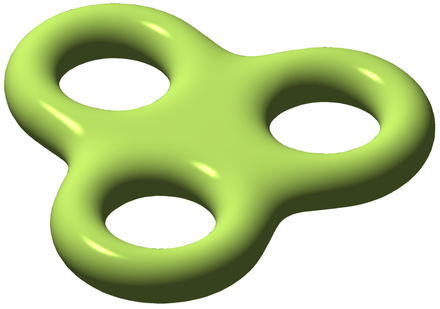
\includegraphics[scale = 1]{RiemannSurface}
**** Riemann Surface of genus 3, from Wikimedia ****

\begin{fact} (Hodge Theory)
The sole topological invariant of a smooth projective curve $C$ is its genus. As a manifold it is a compact, oriented surface, and its genus is half the rank of its first singular cohomology, $H^{1}(C; \CC)$, which is equal to its first deRham cohomology.
Breaking up the deRham cohomology of any smooth complex variety $X$ in terms of holomorphic and antiholomorphic differential
forms we get the \emph{Hodge decomposition}
$$
H^i(X,\CC) = H^i_{\rm de Rham}(X) = \bigoplus_{j=0}^i H^j(\bigwedge^{i-j} \Omega_X).
$$
For a smooth curve $C$, this says in  particular that
$$
H^1(C; \CC) = H^0(\omega_C)\oplus H^1(\sO_C) = H^0(\omega_C)\oplus (H^0(\omega_C))^\vee, 
$$
so $ h^0(\omega_C)$ is half the rank of the middle singular cohomology group, justifying the name ``genus''.
\end{fact}


If $E$ is a divisor of negative degree then $H^0(E) = 0$ so we get the form of the Riemann-Roch theorem
originally proved by Riemann:

\begin{corollary}\label{nonspecial RR}
For any divisor $D$ of degree $d$ we have
$$
h^0(D) \geq d - g + 1,
$$
with equality if $d > 2g-2$.
\end{corollary}
It was Riemann's student Roch  who supplied the correction term $h^0(K_C - D)$ for divisors of lower degree.
The dimension $h^0(K_C-D) = h^1(D)$ was called the \emph{superabundance} of $D$.

Corollary~\ref{nonspecial RR} and Proposition~\ref{very ample} together show that all high degree divisors come from hyperplane sections in 
suitable embeddings:

\begin{corollary}\label{degree 2g+1 embedding}
Let $D$ be a divisor of degree $d$ on a smooth, connected projective curve of genus $g$. If $d \geq 2g$, the complete linear series $|D|$ is basepoint free; and if $d \geq 2g+1$ the associated morphism $\phi_D : C \to \PP^{d-g}$ is an embedding, so that
$D$ is the preimage of the intersection of $C$ with a hyperplane in $ \PP^{d-g}$.
\end{corollary}

Since the complement of a hyperplane in projective space is an affine space, we get an affine embedding result too:

\begin{corollary}
 If $C$ is any smooth, connected projective curve and $\emptyset \neq \Gamma \subset C$ a finite subset then $C \setminus \Gamma$ is affine.
\end{corollary}
\begin{proof}
Let $D$ be the divisor defined by $\Gamma$. By Corollary~\ref{degree 2g+1 embedding} a high multiple of $D$ is very ample,
and gives an embedding $\phi: C\to \PP^n$ such that the preimage of the intersection of $C$ with some hyperplane $H$
is a multiple of $D$. It follows that $C\setminus \Gamma$ is embedded in $\AA^n = \PP^n\setminus H$.
\end{proof}
 
We can  use Corollary~\ref{nonspecial RR} to determine the Hilbert polynomial of a projective curve. To do this, let $C \subset \PP^r$ be a smooth curve of degree $d$ and genus $g$, and consider the exact sequence of sheaves
$$
0 \rTo \cI_{C/\PP^r}(m) \rTo \cO_{\PP^r}(m) \rTo \cO_C(m) \rTo 0
$$
and the corresponding exact sequence
$$
 H^0(\cO_{\PP^r}(m)) \rTo^{\rho_m} H^0(\cO_C(m)) \rTo H^1(\cI_{C/\PP^r}(m)) \rTo 0.
$$

The \emph{Hilbert function} $h_C$ of $C$  is defined by
$$
h_C(m) = \dim_{\CC} (S_{C})_{m} = \rank(\rho_m),
$$
where $(S_{C})_{m}$ is the degree $m$ component of the homogeneous coordinate ring of $C$ in $\PP^n$.

By Theorem~\ref{Serre vanishing} we have $H^1(\cI_{C/\PP^r}(m)) = 0$ for large $m$, so $h_{C}(m) = h^0(\cO_C(m))$ for large $m$, which, by the Riemann-Roch theorem, equals $md-g+1$, again for large $m$. Thus, the Hilbert polynomial of $C \subset \PP^r$ is $p_C(m) = dm-g+1$. 
More generally, we define what is called the \emph{arithmetic genus}:

\begin{definition}\label{genus Hilbert}\label{pa}\label{genus formula}
If $C\subset \PP^n$ is a purely 1-dimensional projective scheme with Hilbert polynomial
$p_C(m) = \chi(\sO_C(m)$, the \emph{arithmetic genus} of $p_a(C)$ is $1-p_C(m)$. If $C$ is integral, then
the \emph{geometric genus} $g(C)$ is the genus of the normalization of $C$.
\end{definition}
We see from the Riemann-Roch theorem that if $C$ is smooth, then $p_a(C) = g(C) = h^0(\omega_C)$, the genus of $C$. In general, we
will see that for integral curves $p_a(C) \geq g(C)$, with equality only when $C$ is smooth.
 
The Riemann-Roch formula does \emph{not} give us a formula for the dimension $h^0(D)$ when $h^0(K_C - D)>0$; such divisors $D$ are called \emph{special divisors}. The existence or non-existence of divisors $D$ with given $h^{0}(D)$ and $h^{1}(D)$ often serves to distinguish one curve from another, and will be an important part of our study.

\subsection{Residues, and a complex-analytic argument for the Riemann-Roch theorem.}\label{RR by residues}

We remarked at the beginning of Chapter~\ref{linear series} that a smooth projective curve over $\CC$ is the same thing as a compact Riemann surface. In this section, we'll adopt the complex analytic viewpoint, and give an explanation of the Riemann-Roch theorem  (Theorem~\ref{RR theorem}) in a special case. We will use the fact that meromorphic functions on a Riemann surface are exactly the rational functions on the corresponding
algebraic curve. We will prove:

\begin{theorem}
Let $X$ be a compact Riemann surface of genus $g$, and let $D = \sum a_i p_i$ be an effective divisor ($=$ formal sum of points $p_i$ with integral coefficients $a_i\geq 0$) of degree $d:= \sum a_i$ on $X$, and suppose that $K-D$ is also effective for some canonical divisor $K$.
The dimension of the space $L(D)$ of meromorphic functions on $X$ with poles of order $a\leq a_i$ at $p_i$ and no other poles, is
$d-g+1$ plus $L(K-D)$, the number of holomorphic differential forms vanishing on each $p_i$ to order at least $a_i$. 
\end{theorem}

We will prove this using residues, under the additional assumption that  $D$ and $K-D$ are both effective (that is, $D$ is both effective and \emph{special} in the sense that there are nonzero functions
both in $L(D)$ and in $L(K-D)$.)

Recall that the \emph{residue} of a meromorphic 1-form $\phi$ at a pont $p$ on $X$ is defined by an integral: choose a disc $\Delta \subset X$ containing $p$ and in which $\phi$ is holomorphic except for its pole at $p$. The residue ${\rm Res}_p(\phi)$ is $\frac{1}{2\pi i}$ times the integral of $\phi$ along the boundary of $\Delta$. If $z$ is a local coordinate on $\Delta$ zero at $p$ and we write the differential $\phi$ as
$$
\phi = \sum_{n=-N}^\infty a_nz^n dz
$$
then by Cauchy's formula, the residue of $\phi$ at $p$ is the coefficient $a_{-1}$. 

\begin{proposition}\label{residue sum}
 if $\phi$ is a meromorphic differential on a compact Riemann surface $X$, then the sum of the residues of $\phi$
 at all the poles of $\phi$ is 0.
 \end{proposition}
 
\begin{proof}
Apply Stokes' theorem to the complement of the union of small discs around each of the poles of $\phi$.
\end{proof}

Let  $D = \sum_{i=1}^s a_ip_i$ be an effective divisor on $X$, and set $d = \sum a_i =: \deg D$. Locally, a function with a pole of order at most $a_i$ at $p$ may be written in terms of a local coordinate $z$ at $p$ as $\sum_{i=-a_i}^infty c_{i}z^{i} $;
the sum $\sum_{i=-a_i}^{-1} c_{i}z^{i}$ is called its \emph{polar part}.
By the maximum principle, a meromorphic function in $L(D)$ is determined, up to the addition of a constant, by its polar parts at the points $p_i$;. Thus we have $\dim L(D) \leq d+1$.

When is a given collection $c_1,\dots,c_d \in \CC$ the polar parts of a global meromorphic function $f$ on $X$? A necessary condition
is that if $\phi \in L(K)$ is a holomorphic differential on $X$, then
$$
\sum {\rm Res}_{p_i}(f \cdot \phi) = 0.
$$
This gives $g$ linear relations on the $c_i$. However, if $\phi$ is a holomorphic differential vanishing at all the points $p_i$
then the corresponding relation is trivial. Thus the number of linearly independent relations on the polar parts of $f$ is actually $g - \dim L(K-D)$; and we arrive at an inequality
$$
\dim L(D) \leq d + 1 - g + \dim L(K-D).
$$

This is a priori only an inequality. But we can apply the same logic to an effective divisor $K-D$, and we see that
\begin{align*}
\dim L(K-D) &\leq \deg(K-D) + 1 - g + L(K - (K-D)) \\
& = 2g - 2 - d + 1 - g  + L(D) \\
&= g - d - 1 + L(D)
\end{align*}

Adding the two inequalities we have
$$
L(D) + L(K-D) \leq L(D) + L(K-D).
$$
Since the sum of the inequalities is an equality, we conclude that each inequality is also an equality; this is the Riemann-Roch formula
in our special case.

\subsection{Arithmetic genus and geometric genus}
In this section, we'll deal with a  curve $C_0$ that is reduced and irreducible, but not necessarily smooth.
Given $C_0$ there is a birational normalization morphism $\nu: C \to C_0$, and any map of a smooth ($=$normal) curve to $C_0$
factors through $C$. Thus $C_0$ is birational to a unique
smooth curve. The genus of $C$ is called the \emph{geometric genus} of $C_0$.

Most of the results of this book have analogues for singular curves, but this is a topic beyond our scope; for us, singular curves will appear as a useful adjunct to our theory, for example in Chapter~\ref{PlaneCurvesChapter}. %\fix{why doesn't this ref print correctly Chapter 12?}

Applied to any 1-dimensional projective scheme $C_0$, the formula~\ref{genus Hilbert}, define
the \emph{arithmetic genus} $p_a(C_0) = 1-\chi(\sO_{C_0})$ of $C_0$. For some examples with curves that are not
integral, see Exercise~\ref{pa example}.
 
Returning to the case where $C_0$ is reduced and irreducible, we can relate the arithmetic and geometric genera of $C_0$ using the map of sheaves
$$
\cO_{C_0} \to \nu_*\cO_C.
$$
This is injective; the cokernel sheaf will be a skyscraper sheaf supported on the singular points of $C_0$. Denoting this sheaf by $\cF$, we have an exact sequence
$$
0 \to \cO_{C_0} \to \nu_*\cO_C \to \cF \to 0.
$$

The normalization map $\nu: C \to C_0$ is finite, so that the direct images $R^i\nu_*\cO_C$ vanish for $i > 0$; it follows from the Leray spectral sequence~\ref{Leray} that $\chi(\nu_*\cO_C) = \chi(\cO_C)$. Thus
$$
p_a(C_0) - g(C) =  \chi(\cO_{C}) -   \chi(\cO_{C_0}) = \chi(\cF) = h^0(\cF) = \deg(\cF)
$$ 
since the support of $\cF$ is finite.
In other words, the difference between the arithmetic and geometric genera of $C_0$ is the sum of the vector space dimensions of the stalks of $\cF$; colloquially, it's the number of linear conditions a function $f$ on $C$ has to satisfy to be the pullback of a function from $C_0$. The length of the stalk of $\cF$ at a particular singular point $p \in C_0$ is called the \emph{$\delta$-invariant} $\delta_p$ of the singularity; to rephrase the statement above in these terms, we have:
$$
p_a(C_0) - g(C) = \sum_{p \in (C_0)_{\rm sing}} \delta_p
$$ 

\begin{proposition}\label{Leray}
 We have used an almost trivial part of the Leray spectral sequence, and we shall use it again in a few other almost equally simple cases. Suppose that $f:X\to Y$ is a morphism of varieties or schemes
 and $\sF$ is a coherent sheaf on $X$.
  It follows immediately from the definition of the push-forward that $\HH^0(\sF) \cong \HH^0(f_*(\sF))$. Replacing
  $\sF$ by an injective or flasque resolution, we get the Leray spectral sequence
  $$
  \HH^p(R^qf_*(\sF)) \Longrightarrow \HH^{p+q}(\sF)
  $$
This is a special case of the spectral sequence for the derived functors of a composite functor ($H^0$ composed with $f_*$);
see~\cite[II.4.17.1]{Godement} or \cite[Section III.7]{Gelfand-Manin} for proofs. \qed
 \end{proposition}

The $\delta$ invariant is easy to compute in simple cases:
\begin{enumerate}

\item (nodes) If $p \in C_0$ is a node, with points $r,s \in C$ lying over it, the condition for a function $f$ on $C$ to descend is simply that $f(r)=f(s)$; this is one linear condition so $\delta_p = 1$.

\item (cusps) If $p \in C_0$ is a cusp, with  $r \in C$ lying over it, the condition for a function $f$ on $C$ to descend is simply that the derivative $f'(r)=0$; again, this is one linear condition so $\delta_p = 1$.

\item (tacnodes) Suppose now that $p \in C_0$ is a \emph{tacnode}, that is, $C_0$ has two smooth branches at $p$ simply tangent to one another. There will be two points $r, s \in C$ lying over it, and the condition for a function $f$ on $C$ to descend is that in terms of suitable local coordinates both $f(r)=f(s)$ and $f'(r)=f'(s)$.  This represents two linear conditions, so $\delta_p = 2$.

\item (planar triple points) An ordinary triple point $p \in C_0$ of a plane curve is a singularity consisting of three smooth branches meeting pairwise transversely, such as the zero locus of $y^3-x^3$. There will be three points $r,s,t \in C$ lying over $p$, and certainly a necessary condition for a function $f$ on $C$ to descend is that $f(r)=f(s)=f(t)$---two linear conditions. But there's a third, less obvious linear condition: in order for $f$ to descend, the derivatives $f'(r), f'(s), f'(t)$ have to satisfy a linear condition---a reflection of the fact that a function on $C_0$ cannot vanish to order 2 on each of two branches without vanishing to order 2 along the third as well. Thus $\delta_p = 3$

\item (spatial triple points) We will be concerned in what follows only with planar singularities, but spatial triple points provide a useful contrast to the last example. A spatial triple point is a singularity consisting of three smooth branches, with linearly independent tangent lines, so that its Zariski tangent space is 3-dimensional. An example would be the union of the three coordinate axes in $\AA^3$.

In this case, in contrast to case of the planar triple point, the condition that $f(r)=f(s)=f(t)$ is both necessary and sufficient for $f$ to descend, and thus  $\delta_p=2$.

\end{enumerate}




\section{The canonical morphism}

 The canonical sheaf on $\PP^1$ has negative degree, so $|K_{\PP^1}| = \emptyset$. In the case $g=1$ the canonical sheaf has degree 0 and since it has nonzero global sections, 
 $\omega_C = \sO_C$, and $K_C = 0$. Thus in studying the canonical series we restrict our attention to curves $C$ of genus $g\geq 2$. 
 
 \begin{theorem}\label{canonical series is very ample} Let $C$ be a smooth curve of genus $\geq 2$.
\begin{enumerate}
 \item $|K_C|$ is basepoint free.
 \item $|K_C|$ is very ample if and only if $C$ admits no map of degree 2 to $\PP^1$.
\end{enumerate}
\end{theorem}

Recall that a curve of genus $\geq 2$
is said to be \emph{hyperelliptic} if there exists a morphism $f: C \to \PP^1$ of degree 2. 
It is easy to describe this in terms of linear series:

\begin{lemma}\label{deg 2 morphism}
Let $C$ be a smooth, projective curve of genus $g\geq 2$. If $C$ has an invertible sheaf $\cL$ of degree $\leq 2$ with two independent sections, then $\cL$ has degree 2 and
$|\cL|$ defines a morphism of degree 2 to $\PP^{1}$, so if $g(C)\geq 2$ then $C$ is hyperelliptic. In particular, if $g(C) = 2$ then the canonical series $|K_{C}|$ defines a 2 to 1 morphism to $\PP^{1}$, so $C$ is hyperelliptic.
\end{lemma}

\begin{proof}
Since $C \not\cong \PP^1$,  Theorem~\ref{characterization of P1} shows that $C$ cannot have a 1-dimensional linear series
of degree $< 2$. Thus $\sL$ has degree exactly 2, and no basepoints, so it defines a morphism of degree 2 to $\PP^1$ as claimed.
\end{proof}

\begin{proof}[Proof of Theorem~\ref{canonical series is very ample}]
A point $p$ is a basepoint of $|K_C|$ if and only if $h^0(K_C-p) = h^0(K_C) = g$. By the Riemann-Roch theorem,
this is eqivalent to $h^0(p) =2$, which would imply that $C\cong \PP^1$ by Theorem~\ref{characterization of P1}. Thus $K_C$
has no basepoints.

By Proposition~\ref{very ample} we have to show that for any pair of points $p, q \in C$ we have
$$
h^0(K_C(-p-q)) = h^0(K_C)-2 = g-2.
$$
Applying \trr we see this fails if and only if $h^0(\cO_C(p+q)) \geq 2$ for some $p,q \in C$. By Lemma~\ref{deg 2 morphism}, this implies that $C$ is hyperelliptic. Conversely, if $C$ is hyperelliptic then for some divisor $D = p+q$ we have $h^0(D) = 2$, whence $h^0(K-p-q) = h^0(K) -1$ by
the Riemann-Roch formula.
\end{proof}

The image of the canonical morphism of a non-hyperelliptic curve of genus $g>2$ is called a \emph{canonical curve}.


\subsection{The geometric Riemann-Roch theorem}

If $C$ is a smooth curve of genus $g\geq 2$ we write $\phi_K: C\to \PP^{g-1}$ for the canonical morphism.
If  $D = p_1+\dots + p_d$ is a divisor on $C$ of degree $d$, we will write $\overline{ \phi_K(D)}$ for the \emph{span}
of  $\phi_K(D)$, that is, the dimension of the smallest  subspace of $\PP^{g-1}$ containing $\phi_K(D)$. Since the hyperplanes in $\PP^{g-1}$ containing $\phi_K(D)$ correspond (up to scalars) to sections of $K_C$ vanishing on $D$, we see that
$$
h^0(K_C-D) = \codim \overline{ \phi_K(D)} \subset \PP^{g-1}= g - 1 - \dim \overline{ \phi_K(D)}.
$$
Applying the Riemann-Roch theorem we obtain  the \emph{geometric Riemann-Roch theorem}:

\begin{corollary}\label{geometric RR}
If $D$ is a divisor on a smooth curve $C$ of genus $\geq 2$ then
$$
r(D) = d - 1 - \dim \overline{ \phi_K(D)}.
$$
\end{corollary}

When $C$ is not hyperelliptic, $\phi_K$ is an isomorphism, and we say that $ \phi_K(C)\subset \PP^{g-1}$ is \emph{canonically embedded}. In this case, supposing for simplicity that $D = p_1+\cdots+p_d$ is a sum of distinct points, we can say that the dimension of the linear series $|D|$  is equal to the number of linear relations between the points $p_i$ on the canonical curve. 

\subsection{Linear series on a hyperelliptic curve}
We can describe the canonical map of a hyperelliptic curve---and indeed all its special linear series---quite precisely:

\begin{corollary}\label{canonical on hyperelliptic}
Let $C$ be a smooth hyperelliptic curve of genus $g\geq 2$. The curve $C$ admits a unique degree 2 morphism $\pi: C\to \PP^1$,
and the canonical map $\phi_K: C\to \PP^{g-1}$ is the composition of $\pi$ with the Veronese map of degree $g-1$ from
$\PP^1$ to the rational normal curve of degree $g-1$; that is, every canonical divisor is a sum of $g-1$ fibers of $\pi$.
\end{corollary}

\begin{proof}
If $D$ is a general fiber of a degree 2 map $\pi:C\to \PP^1$ so that $D= p+q$ and $r(D) = 1$, then by the Riemann-Roch theorem or its geometric version, $D$ imposes only one condition on sections of $K_C$; that is, $\phi_K(p) = \phi_K(q)$. Consequently the degree of the canonical morphism $\phi_K$ is at least 2, and the image is thus a nondegenerate curve in $\PP^{g-1}$ of degree $\leq (2g-2)/2 = g-1$. By Theorem~\ref{characterization of P1}, the image of $\phi_K$ is the rational normal curve of degree $g-1$ and every fiber of $\phi_K$ is a divisor linearly equivalent to $D$. It follows that $\pi$ is determined by $K$, so it is unique. Since every canonical divisor is the pullback of a hyperplane section of the rational normal curve,
every canonical divisor is a sum of $g-1$ fibers of $\pi$.
\end{proof}

We can use these ideas to analyze all special divisors.

\begin{corollary}\label{special on hyperelliptic} Let $C$ be a smooth hyperelliptic curve with map $\pi: C\to \PP^1$ of degree 2.
Every special divisor $D$ of degree $d$ on a hyperelliptic curve is a sum of $s$ fibers of $\pi$ and $d-2s$ basepoints.
\end{corollary}

\begin{proof}
Suppose that $D$ contains the sum $E$ of $s$ fibers of $\pi$ and no more; and write $D = E+D'$, with $\deg D' = d-2s$.
 
If $\phi_K:C \to \PP^{g-1}$ is the canonical map, then $\phi_K(D')$ consists of $d-2s$ distinct points, while $\phi_K(E)$ consists of
$s$ points. By Corollary~\ref{independence of points on a RNC} the span of $\phi_K(D)$ has dimension $\min\{g-1, d-s-1\}$, so 
$r(D) = d-1-\min\{g-1, d-s\} = \max \{s,d-g\}$. Since $D$ is a special divisor, $r(D) > d-g$, so $r(D) = s$. 
Since $r(E) =s$, we see that $D'$ is in the base locus of $D$.
\end{proof}

\section{Clifford's theorem}

While the Riemann-Roch Theorem gives a lower bound for the dimension of a linear series, $r(\sL) := h^0(\sL)-1 \geq \deg \sL -g$, Clifford's Theorem
gives an upper bound. If $\deg \sL>2g-2$, then the Riemann-Roch inequality becomes an equality, so it is enough to treat the case $\deg \sL \leq 2g-2$. The bound is actually a corollary of the Riemann-Roch theorem.

\begin{corollary}\label{Clifford bound}
 Let $C$ be a curve of genus $g$ and $\cL$ a line bundle of degree $d \leq 2g-2$. Then
$$
r(\cL) \leq \frac{d}{2}.
$$
\end{corollary}

\begin{proof}
If $\cL$ is nonspecial then, since $g\geq d/2 + 1$, we have $r(\cL) = d-g+1\leq d/2$.
Otherwise we have
$$
r(K_C\otimes \cL^{-1}) = r(\cL) +g - d - 1
$$
by the Riemann-Roch Theorem,
and so by Proposition~\ref{sum of linear series}
$$
g = r(K_C)+1  \geq r(\cL) + r(K_C\otimes \cL^{-1}) +1  = 2r(\cL) +g - d;
$$
hence $r(\cL) \leq d/2$.
\end{proof}

The usual statement of Clifford's theorem includes a description of when equality can occur:

\begin{theorem}\label{Clifford}\label{Clifford equality}
Let $C$ be a curve of genus $g$ and $\cL$ a line bundle of degree $d \leq 2g-2$. If
$$
r(\cL) = \frac{d}{2},
$$
the largest possible value, then either
\begin{enumerate}
\item $d=0$ and $\cL = \cO_C$;
\item $d = 2g-2$ and $\cL = K_C$; or
\item $C$ is hyperelliptic, and $|\cL|$ is a multiple of the $g^1_2$ on $C$.
\end{enumerate}
\end{theorem}

From Corollary~\ref{canonical on hyperelliptic} and Corollary~\ref{geometric RR} we see that the equality does indeed hold
in each of the cases enumerated. Clifford's Theorem is true for smooth curves over fields of any characteristic (see for example \cite[IV.5.4]{Hartshorne1977}, but in characteristic 0 it is a simple consequence of the much more 
Corollary~\ref{Clifford equality plus}
that we will prove via the Uniform position lemma.


 \section{Curves on surfaces}
 We will often analyze curves  on a smooth surface. Compared to the theory of linear series on curves, there is a new element: the intersection pairing. We refer to~\cite[Chapter V]{Hartshorne1977}
 and~\cite[Chapter I]{Beauville} for proof of the unproven statements in this section.
 
 We suppose for this section that $X$ is a smooth projective surface.
 We define $\Pic(X)$ to be the group whose elements are invertible sheaves on $X$.
When two divisors $D,E$ on $X$ meet transversely we define $D\cdot E$ to be the number of points in which they meet. If they have no common
components, we can still define a non-negative intersection multiplicity $m_X(D,E,p)$ at each point $p$, and then set
$$
D\cdot E = \sum_p m_X(D,E,p).
$$
Over the complex numbers each codimension 1 subvariety $D$ of $X$ has a fundamental class
$[D]\in H^2(X, \ZZ)$ and the product is the cup product with values in $H^4(X,\ZZ)$, which is $\ZZ$ since $X$ is compact and orientable. Thus
there is an extension of the product to the cases where $D,E$ have common components. From a geometric point of view, we may choose an
appropriate $C^\infty$
normal vector field along $E$ and define $E'$ by ``pushing'' $E$ out slightly along the direction of this field, until $D$ and $E'$ are transverse,
and the intersections can be computed in the usual way. It should be noted that such intersection numbers can be either positive or negative,
since they depend on the relative orientations of $D$ and $E'$ at the intersection points; this is in contrast to the case when $D$ and $E$
themselves meet properly; in this case the fact that the complex numbers are canonically oriented makes the intersection number non-negative.

The intersection product can also be defined algebraically, over any field, for the intersection of Cartier divisors,
on any surface, even when the surface is singular: Setting $\sL := \sO_X(C)$ and
$\sM := \sO_X(D)$ to simplify the notation, we set 
$$
D\cdot E = \chi(\sO_X)-\chi(\sL^{-1}) -\chi(\sM^{-1}) +\chi(\sL^{-1}\otimes \sM^{-1}) 
$$
\begin{theorem} The pairing $(D,E) \mapsto (D\cdot E)$ is the unique bilinear map
$\Pic(X) \times \Pic(X) \to \ZZ$ extending the case of intersections of two transverse curves on $X$. 
\end{theorem}

A frequent use of the the intersection pairing is to compute the (arithmetic) genus of a curve on a surface,
a result called the adjunction formula.

\begin{theorem}[Adjunction Formula]\label{adjunction formula} \cite[Theorem ****]{Hartshorne1977}
If $C$ is a Cartier divisor  on a complete intersection $X\subset \PP^n$ of any dimension, then 
$$
\omega_C = \omega_X \otimes \sO_X(C) \otimes \sO_C;
$$
in particular, 
\begin{enumerate}
 \item If $X\subset \PP^n$ is the complete interesection of divisors of degree $d_1, \dots, d_c$, then
 $\omega_X = \sO_X( \sum_1^c d_i -n-1).$
 \item If $C$ is a Cartier divisor on surface $X$ that is a complete intersection
in $\PP^n$ then: \label{genus formula}
$$
p_a(C) = \frac{(K_X+C)\cdot C}{2} +1.
 $$
\end{enumerate}
\end{theorem}

We will frequently be interested in curves on quadrics in $\PP^3$, and we can spell out the
intersection theory on these surfaces very concretely; see for example~\cite[Section V.1]{H}.
We will treat them and the curves on them in detail in Section~\ref{curves on scrolls} as part of the larger family of 2-dimensional rational normal scrolls; for
now we sketch the situation as an example of the theory of this section. 

\begin{example}[Quadrics in $\PP^3$]\label{Div of quadric}
 
Quadric surfaces $S$ in $\PP^3$ are classified by their rank:
\begin{itemize}
\item A quadric of rank 1 is a double plane, defined by the square of a linear form;
a quadric of rank 2 is the union of two planes; thus a nondegenerate irreducible curve cannot be contained in a quadric of rank 1 or 2.
\item A rank 3 quadric $S$ is a cone over a plane conic. If $C$ is a smooth,
curve on such a quadric, then:
\begin{itemize}
\item  If $C$  does
not pass through the vertex then it is the intersection of the quadric with a hypersurface of some
degree $d$. In this case $C$ has degree $2d$ and genus $(d-1)^2$. 
 \item If $C$ passes through the vertex, then $C$ lies in the divisor class of a line through the origin plus the intersection of $S$ with a hypersurface of some degree $d$. In this case $C$ has degree $2d+1$ and 
 genus $d(d-1)$. 
\end{itemize}

\item A quadric of rank 4 is nonsingular, and is isomorphic to $\PP^1\times \PP^1$.

\item The Picard group of $\PP^1\times \PP^1$ is $\ZZ\oplus \ZZ$, generated by the 
classes of the lines $\{p\}\times \PP^1$ and $\PP^1\times \{p\}$, where $p\in \PP^1$
is any point. These lines have self-intersection 0, and meet transversely in a point,
so the intersection pairing is given by $(a,b)\cdot(c,d) = ad+bc$. Let $H$ be a 2-plane in $\PP^3$.
Treating 
the quadric $Q$ as a divisor $2H$ in $\PP^3$, we can use the adjunction formula on $\PP^3$
to see that the canonical divisor $K_Q$ is the restriction of $-2H$ to $Q$, that is, a divisor of type $(-2,-2)$.
Applying the adjunction formula again to a divisor $C$ of type $(a,b)$ on $Q$, we see
that the arithmetic genus of $C$ is
$$
\left(((a,b)+(-2,-2))\cdot (a,b)\right)/2 +1 = (a-1)(b-1).
$$

\item Writing $\pi_1, \pi_2$ for the two projections of
$\PP^1\times \PP^1 \to \PP^1$, the sheaf 
$$
\sL := \sO_{\PP^1\times \PP^1}(a,b) = \pi_1^*\op1a \otimes \pi_2^*\op1b
$$
has cohomology given by the K\"unneth formula, for example
\begin{align*}
 H^0(\sL) &= H^0(\op1a)\otimes H^0(\op1b) \hbox{ and thus }\\
 h^0(\sL) &= (a+1)(b+1) \hbox{ if } a\geq 0, b\geq 0.
\end{align*}

\item Any smooth quadric surface $S\subset \PP^3$ is the 
image of $\PP^1\times \PP^1$ embedded by the complete linear series
$|\sO_{\PP^1\times \PP^1}(1,1)|$ and thus contains two families of lines. 
A curve in the class $(a,b)$ thus has degree $(a,b)\cdot(1,1) = a+b$. 
\end{itemize}
\end{example}

Often we wish to compute the dimension of the space of sections of an invertible sheaf, but
as with the case of curves, the Euler characteristic is more accessible:

\begin{theorem}[Riemann-Roch for surfaces] Let $\sL$ be an invertible sheaf on a smooth surface $S$.
The Euler characteristic $\chi(D) := h^0(\sL)-h^1(\sL)+h^2(\sL)$, where $\sL = \sO_S(D)$, is given by
$$
\chi(D) = \chi(\sO_S) + \frac{(D-K_S)\cdot D}{2}+1
$$
\end{theorem}

%\fix{Possible addition:  the Hodge Index theorem as corollary. This could be used to prove finiteness of the automorphism group of a curve following Hartshorne V Ex. 1.11, perhaps in place of the proof now in the inflections chapter.}

It is useful to know what happens under mappings of surfaces, particularly the case of the mapping
corresponding to blowing up a point.

\begin{theorem}
If $\pi: X \to Y$ is a birational map of smooth surfaces, then the pullback map on divisors
preserves the intersection pairing. If $X$ is the blowup of $Y$ at a point $p$ with exceptional
divisor $E = \pi^{-1}(p)$, then:

\begin{enumerate}
 \item $\Pic X =\pi^*(\Pic Y) \oplus \ZZ E$.
\item The canonical class on $X$ is given by $K_X = \pi^*(K_Y)+E$.
 \item The intersection pairing on $\Pic X$ is given by
 
\begin{itemize}
\item $\pi^*(D)\cdot\pi^*(D') = D\cdot D'$ for all $D,D'\in \Pic Y$.
\item $\pi^*(D)\cdot E = 0$ for all $D\in \Pic Y$.
 \item $E\cdot E = -1$.
 \item $K_X\cdot E = -1$.
 \item If $C$ is a curve that has an $m$-fold point at $p$ then $\pi^{-1}(C)$ contains $E$ with multiplicity $m$.
 \end{itemize}
\end{enumerate}
\end{theorem}

Blowups occur frequently in the theory of surfaces, and are easy to characterize:
\begin{theorem}
If $E\subset X$ is a curve on a smooth projective surface $X$ and
 that $E^2 = E\cdot K_X = -1$ then $E$ can be ``blown down'' in the sense that
 $X$ is the blowup of a smooth surface $Y$ at a point $p\in Y$, and $E$ is the exceptional divisor.
\end{theorem}


\section{Exercises}

In the following series of exercises, we are going to be working with smooth projective curves associated to a given affine curve $C^\circ := V(f(x,y)) \subset \AA^2$; this is the unique smooth projective curve containing the normalization of $C^\circ$ as a Zariski dense open subset.

\begin{exercise}
Let $C$ be the smooth projective curve associated to the affine plane curve $y^3 +x^3 = 1$, and let $\pi : C \to \PP^1$ be the map given by the rational function $x$.
\begin{enumerate}
\item Find the branch points and ramification points of $\pi$, and deduce that the genus of $C$ is 1.
\item For any two points $p, q \in C$ find the complete linear series $|p+q|$.
\item Find the (unique) map $\eta : C \to \PP^1$ of degree 2 such that $\eta((1,0)) = \eta((0,1))$, and determine the ramification points of $\eta$.
\item Show that $C$ is isomorphic to the smooth projective curve associated to the affine plane curve $y^2 +x^3 = 1$.
\end{enumerate}
\end{exercise}

For the next three exercises, let $C^\circ$ be the affine plane curve given as the zero locus of $y^2 - x^6 +1$, and let $C$ be the corresponding smooth projective curve. Note that the map $C^\circ \to \AA^1$ given by the projection $(x,y) \mapsto x$ extends to a map $\pi : C \to \PP^1$, expressing $C$ as a 2-sheeted cover of $\PP^1$ branched over the points $1, \zeta, \dots, \zeta^5$, where $\zeta$ is any primitive 6th root of unity. In addition, let $p$ and $q \in C$ be the two points lying over the point $\infty \in \PP^1$.

\begin{exercise}\label{hyperelliptic curve 1}
Let $C^\circ$ be the affine plane curve given as the zero locus of $y^2 - x^6 +1$, and let $C$ be the corresponding smooth projective curve. 

Show  that the map $C^\circ \to \AA^1$ given by the projection $(x,y) \mapsto x$ extends to a map $\pi : C \to \PP^1$, expressing $C$ as a 2-sheeted cover of $\PP^1$ branched over the points $1, \zeta, \dots, \zeta^5$, where $\zeta$ is any primitive 6th root of unity. Show that there are two distinct points $p$ and $q \in C$  lying over the point $\infty \in \PP^1$,
so that $C$ is unramified over $\infty$.

What is the genus of $C$?
\end{exercise}

\begin{exercise} With $C$ as in Exercise~\ref{hyperelliptic curve 1}:
\begin{enumerate}

\item Let $r_\alpha$ be the branch point over $\zeta^\alpha$. Show that
$$
p+q \sim 2r_\alpha \quad \text{and} \quad \sum_{\alpha = 0}^5 r_\alpha \sim 3p+3q.
$$

\item Find the vector space $H^0(\cO_C(D))$ where $D = r_0 + r_2 + r_4$, and find the (unique) divisor $E$ on $C$ such that $E + r_1 \sim r_0 + r_2 + r_4$.

\end{enumerate}

\end{exercise}

\begin{exercise}
With $C$ as in Exercise~\ref{hyperelliptic curve 1}:
Let $D$ be the divisor $D = p + q + r_0 + r_3$
\begin{enumerate}
\item Find the vector space $H^0(\cO_C(D))$.
\item Describe the map $\phi_{|D|} : C \to \PP^2$.
\item Find the equation of the image curve $\phi_{|D|}(C) \subset \PP^2$, and describe its singularities.
\end{enumerate}
\end{exercise}
 
\begin{exercise}
Let $C$ be the smooth projective curve associated to the affine curve $y^3 = x^5 -1$. Note that the map $\pi : C \to \PP^1$ given by the function $x$ expresses $C$ as a cyclic, 3-sheeted cover of $\PP^1$, branched over the 5th roots of unity and the point at $\infty$. By way of notation, if we take $\eta = e^{2\pi i/5}$ a primitive 5th root of unity, we'll denote by $r_\alpha$ the point $(\eta^\alpha, 0) \in C$ lying over $\eta^\alpha$, and by $p$ the point lying over $\infty \in \PP^1$.

\begin{enumerate}
\item Verify that there is indeed a unique point $p \in C$ lying over $\infty \in \PP^1$, and the map has ramification index 2 at $p$. 
\item Show that the genus of $C$ is 4.
\item Establish the linear equivalences
$$
3p \sim 3r_\alpha \quad \text{and} \quad r_1+ \dots + r_5 \sim 5p.
$$
\item Find a basis for the space $H^0(K_C)$ of regular differentials on $C$.
\item Show that $C$ is not hyperelliptic.
\item Describe the canonical map $\phi_K : C \to \PP^3$ and find the equations of the image.
\item Let $D$ be the divisor $D = r_1+\dots+r_5$. Show that $h^0(K_C(-D)) = 1$; deduce that $r(D) = 2$, and find a basis for $H^0(\cO_C(D))$.
\item If $E = 3p$, show that $r(E) = 1$; that $|E|$ is the unique $g^1_3$ on $C$ and that $2E \sim K$.
\end{enumerate}
\end{exercise}


\begin{exercise}\label{pa example}
\begin{enumerate}
 \item Show that the arithmetic genus of the disjoint union of two lines is $-1$.
\item Let $L\subset Q\subset \PP^3$ be a line on a smooth quadric surface in $\PP^3$. Show that the 
divisor $3L$, regarded as a 1-dimensional scheme, has $p_a(3L) = -2$.
\item Compare these results with the result of simply applying the adjunction formula.
\end{enumerate}
\end{exercise}

\begin{exercise}\label{gonality exclusion}
Show that a curve of genus $g \geq 3$ cannot be simultaneously hyperelliptic and a three-sheeted cover of $\PP^1$.
\end{exercise}

\begin{exercise}\label{planar triple pt}
Show that normalization of the affine planar triple point $xy(x-y) = 0$ in $\AA^2$ is the disjoint union of three
affine lines, $\Spec(\CC[x] \times \CC[y]\times \CC[z]$. Compute the linear conditions on the values and derivatives of three polynomial functions f,g,h defined on
these three lines that they ``descend'' to give a well-defined function on the planar triple point.
\end{exercise}

\begin{exercise} Generalize the results on planar triple points, above, to the case of a plane curve with $n$ pairwise
transverse branches, called an \emph{ordinary multiple point}.
\end{exercise}

\begin{exercise}\label{delta=1 characterization}
Let $p \in C$ be a singular point of a reduced curve $C$. Show that if $\delta_p = 1$, then $p$ must be either a node or a cusp.
\end{exercise}



 %footer for separate chapter files

\ifx\whole\undefined
%\makeatletter\def\@biblabel#1{#1]}\makeatother
\makeatletter \def\@biblabel#1{\ignorespaces} \makeatother
\bibliographystyle{msribib}
\bibliography{slag}

%%%% EXPLANATIONS:

% f and n
% some authors have all works collected at the end

\begingroup
%\catcode`\^\active
%if ^ is followed by 
% 1:  print f, gobble the following ^ and the next character
% 0:  print n, gobble the following ^
% any other letter: normal subscript
%\makeatletter
%\def^#1{\ifx1#1f\expandafter\@gobbletwo\else
%        \ifx0#1n\expandafter\expandafter\expandafter\@gobble
%        \else\sp{#1}\fi\fi}
%\makeatother
\let\moreadhoc\relax
\def\indexintro{%An author's cited works appear at the end of the
%author's entry; for conventions
%see the List of Citations on page~\pageref{loc}.  
%\smallbreak\noindent
%The letter `f' after a page number indicates a figure, `n' a footnote.
}
\printindex[gen]
\endgroup % end of \catcode
%requires makeindex
\end{document}
\else
\fi
